\documentclass[10pt,letterpaper]{article}
\usepackage[top=0.85in,left=2.75in,footskip=0.75in,marginparwidth=2in]{geometry}

% use Unicode characters - try changing the option if you run into
% troubles with special characters (e.g. umlauts)
\usepackage[utf8]{inputenc}

% clean citations
\usepackage{cite}

% hyperref makes references clicky. use \url{www.example.com} 
% or \href{www.example.com}{description} to add a clicky url
\usepackage{nameref,hyperref}

% line numbers
\usepackage[right]{lineno}

% improves typesetting in LaTeX
\usepackage{microtype}
\DisableLigatures[f]{encoding = *, family = * }

% text layout - change as needed
\raggedright
\setlength{\parindent}{0.5cm}
\textwidth 5.25in 
\textheight 8.75in

% Remove % for double line spacing
%\usepackage{setspace} 
%\doublespacing

% use adjustwidth environment to exceed text width (see examples in text)
\usepackage{changepage}

% adjust caption style
\usepackage[aboveskip=1pt,labelfont=bf,labelsep=period,singlelinecheck=off]{caption}

% remove brackets from references
\makeatletter
\renewcommand{\@biblabel}[1]{\quad#1.}
\makeatother

% headrule, footrule and page numbers
\usepackage{lastpage,fancyhdr,graphicx}
\usepackage{epstopdf}
\pagestyle{myheadings}
\pagestyle{fancy}
\fancyhf{}
\rfoot{\thepage/\pageref{LastPage}}
\renewcommand{\footrule}{\hrule height 2pt \vspace{2mm}}
\fancyheadoffset[L]{2.25in}
\fancyfootoffset[L]{2.25in}

% use \textcolor{color}{text} for colored text (e.g. highlight to-do areas)
\usepackage{color}

% define custom colors (this one is for figure captions)
\definecolor{Gray}{gray}{.25}

% this is required to include graphics
\usepackage{graphicx}

% use if you want to put caption to the side of the figure 
% see example in text
\usepackage{sidecap}

% use for have text wrap around figures
\usepackage{wrapfig}
\usepackage[pscoord]{eso-pic}
\usepackage[fulladjust]{marginnote}
\reversemarginpar

% document begins here
\begin{document}
\vspace*{0.35in}

% title goes here:
\begin{flushleft}
{\Large
\textbf\newline{Optimizing bead-based T cell activation through computational
                modeling}
}
\newline
% authors go here:
\\
Bulent Arman Aksoy\textsuperscript{*},
Eric Czech\textsuperscript{*},
Jeff Hammerbacher\textsuperscript{*}
\\
\bigskip
{*} Medical University of South Carolina,
       Department of Microbiology and Immunology,
       Charleston, SC, 29425
\end{flushleft}

\section*{Abstract}
Short- and long-term culturing of the T cells for research or clinical purposes rely on continuous expansion of these cells.
Without activation, T cells do not proliferate efficiently and on top of that, their inactive profile makes them harder to manipulate and profile.
Commonly used activation techniques are similar to each other in principle but the specific method used for T cell activation can enrich certain T subsets.
Anti-CD3- and anti-CD28-based activation is the most commonly used technique in both research and clinical settings.
Since this method is not antigen-specific, it does not lead to rapid clonal expansion but instead helps maintain the proliferation of a diverse set of T cells.

% now start line numbers
\linenumbers

% the * after section prevents numbering
\section*{Introduction}

%\clearpage

\section*{Results}

\begin{figure}[ht]
    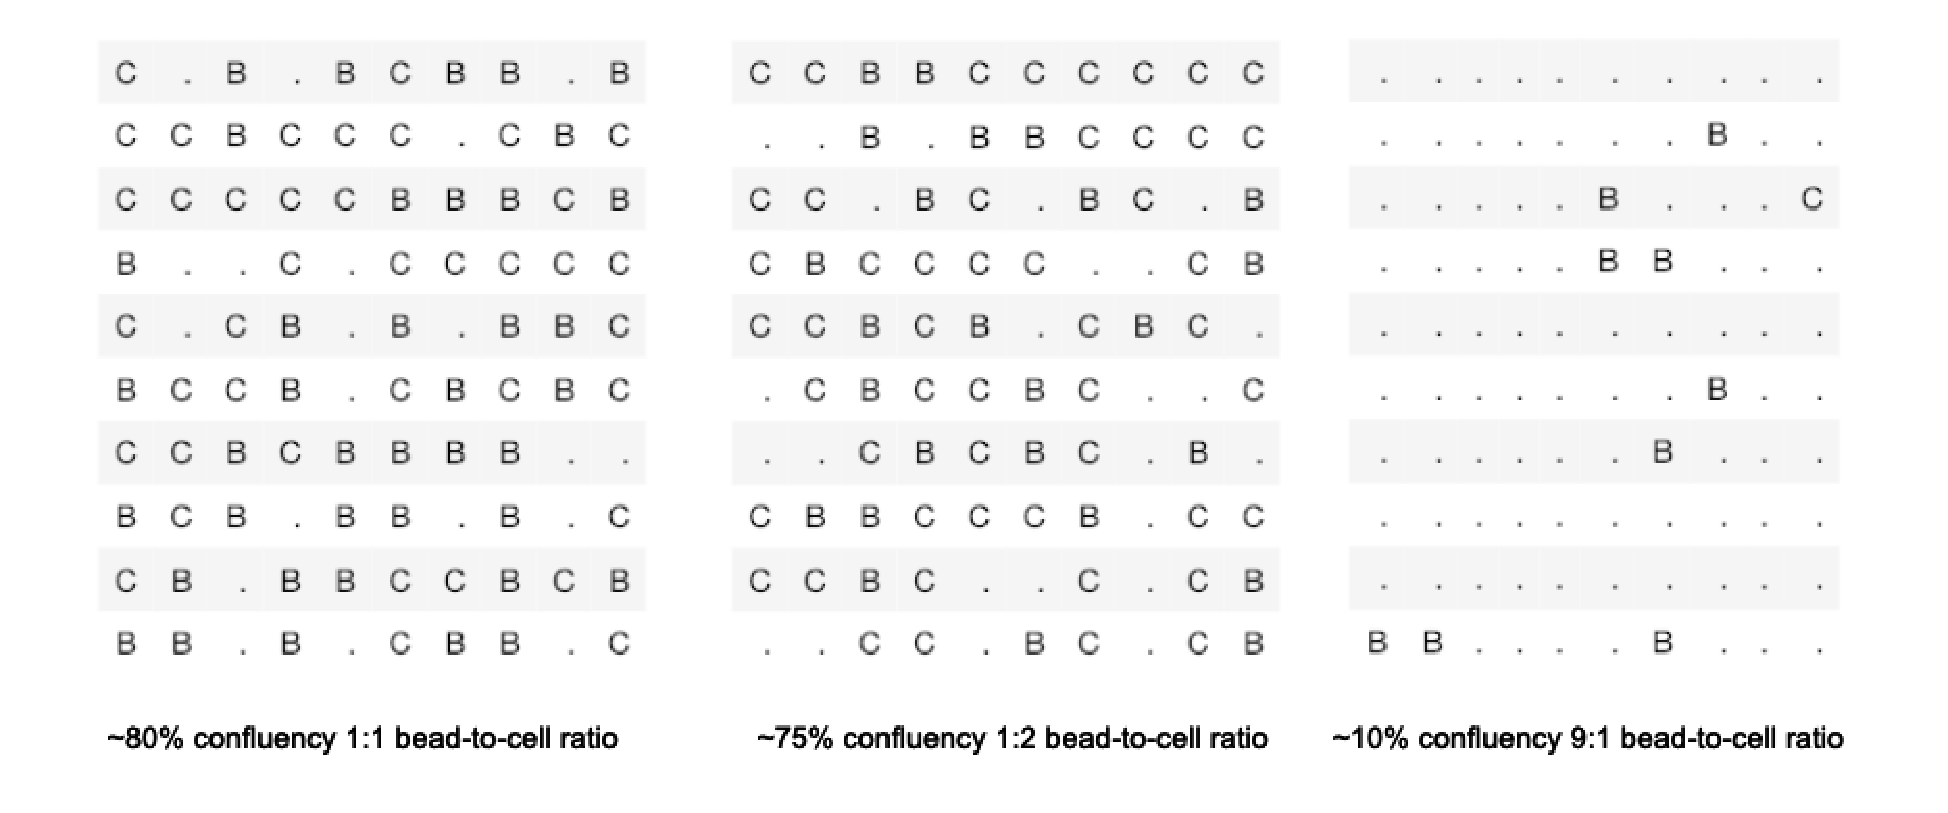
\includegraphics[width=\textwidth]{fig-simulations-samples.pdf}
    \caption{
        \color{Gray} \textbf{Virtual culture plates}.
        With that said, let's try to simulate this in silico. Assume that our virtual plate is 10-by-10 so it has a total of 100 slots. Each cell can be only one of the following: bead (B), cell (C), or empty (E). We can decide how many of these slots we will be using when creating a virtual plate but the assignments will be completely random.
    }
    \label{fig-simulations}
\end{figure}


\begin{figure}[ht]
    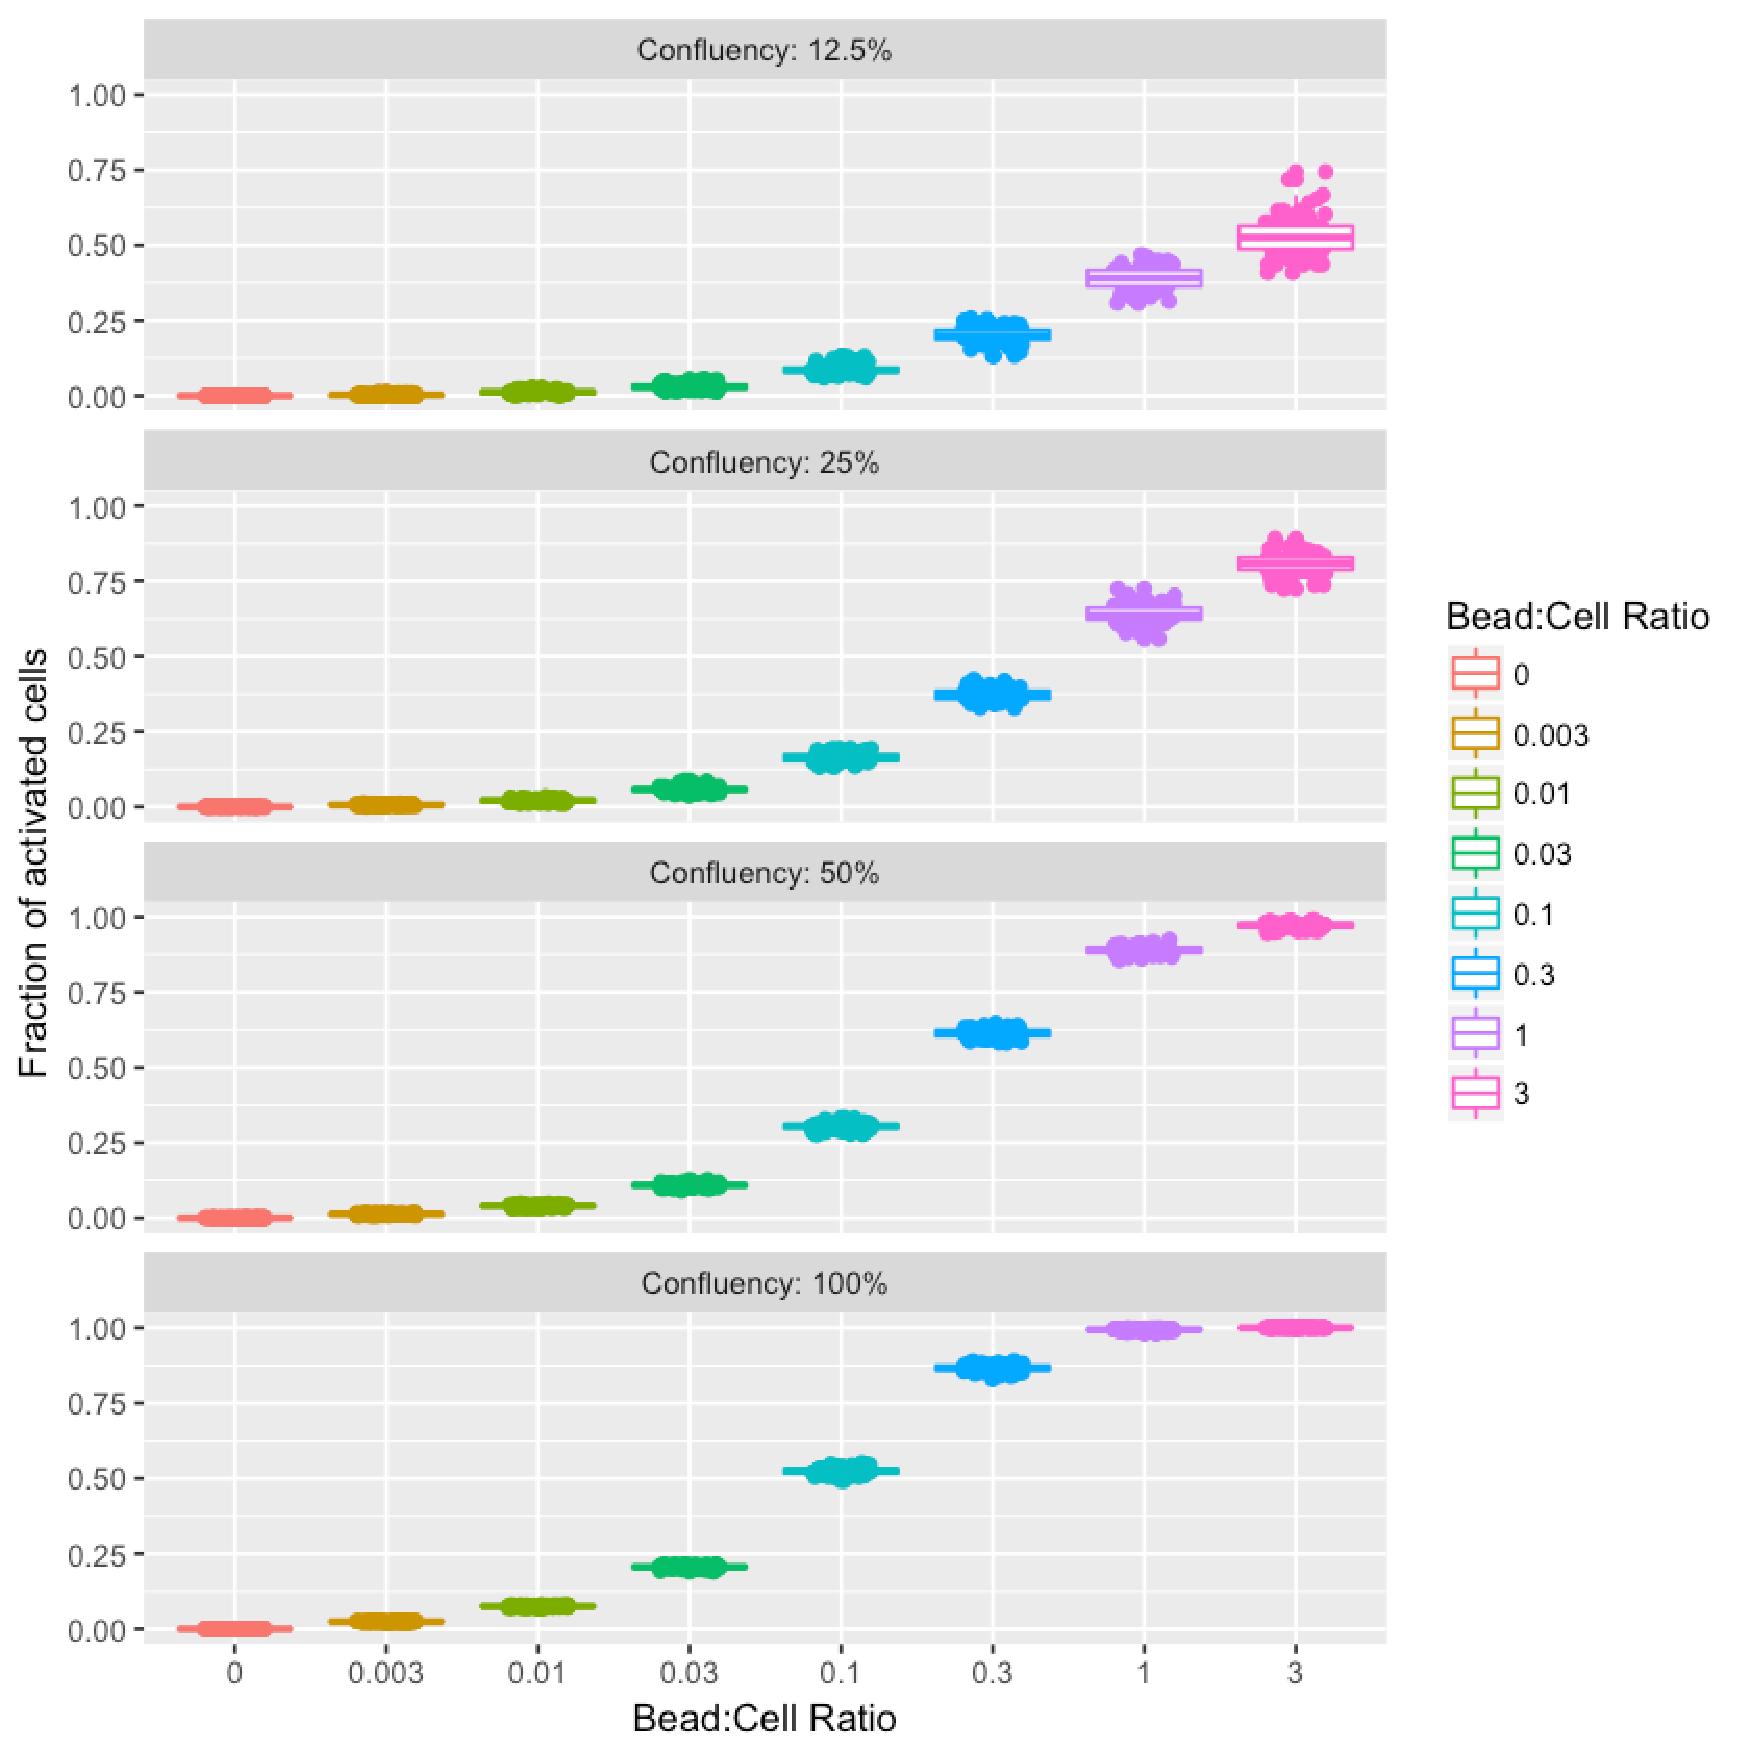
\includegraphics[width=\textwidth]{fig-simulations.pdf}
    \caption{
        \color{Gray} \textbf{Simulating different conditions}.
        This is amazing! One thing that is apparent from this experiment is that the efficiency of activation, as defined by the fraction of cells that are activated, depends on both the bead:cell ratio and the confluency. At a higher confluency, a cell ending up near a bead is much more likely hence even with fewer bead (0.3), we almost always get ~90\% activation. As the confluency goes down, the efficiency also goes down so for example, using 3 beads to 1 cell at 25\% confluency can barely activate 75\%.
    }
    \label{fig-simulations}
\end{figure}

\section*{Acknowledgments}
We thank just about everybody.

\nolinenumbers

%This is where your bibliography is generated. Make sure that your .bib file is actually called library.bib
\bibliography{library}

%This defines the bibliographies style. Search online for a list of available styles.
\bibliographystyle{abbrv}

\end{document}

